\documentclass[10pt,twocolumn]{article}

\usepackage[letterpaper,top=0.82in,bottom=0.88in,left=0.68in,right=0.68in,columnsep=0.26in]{geometry}
\usepackage{mathptmx}
\usepackage{microtype}
\usepackage{amsmath,amssymb,amsthm}
\usepackage{booktabs}
\usepackage{multirow}
\usepackage{enumitem}
\usepackage{xcolor}
\usepackage{tikz}
\usetikzlibrary{arrows.meta,positioning,shapes.geometric,fit,calc,backgrounds}
\usepackage{pgfplots}
\pgfplotsset{compat=1.18}
\usepackage[colorlinks=true,linkcolor=blue!65!black,citecolor=teal!70!black,urlcolor=blue!70!black]{hyperref}

\newtheorem{proposition}{Proposition}
\newtheorem{remark}{Remark}

\definecolor{hostblue}{RGB}{28,93,153}
\definecolor{forgered}{RGB}{186,45,45}
\definecolor{stemteal}{RGB}{22,128,112}
\definecolor{moepurple}{RGB}{106,61,154}
\definecolor{shdcgold}{RGB}{196,125,14}

\title{\Large\textbf{HoST-MoE: Host-Differential Spatio-Temporal Mixture of Experts for\\Unified Detection and Localization of AI-Manipulated Videos}}

\author{
  Lucas Brand\~{a}o\\
  {\small Code, Configs \& Reproducibility Suite: \texttt{host-forensics} (Apache-2.0)}
}
\date{}

\begin{document}
\maketitle

\begin{abstract}
Modern AI video manipulation tools---spanning zero-shot identity swaps, implicit-keypoint portrait reenactment, latent-diffusion lip-sync dubbing, flow-guided object removal, and sparse audio-visual splices---modify localized regions or intervals inside authentic camera-captured footage rather than synthesizing entire videos from scratch. Yet existing forensic detectors remain fragmented across incompatible paradigms: parameter-efficient ViT adapters collapse across spatial-versus-temporal manipulation families, multimodal LLM localizers miss low-level inpainting traces ($0.135$ mIoU on object removal) at prohibitive latency (${\sim}16$\,s/clip), entangled audio-visual fusion bleeds false alarms across tracks, and uncalibrated logits suffer severe cross-domain score polarization under codec and neural-restoration shifts. We introduce \textbf{HoST-MoE} (\emph{Host-Differential Spatio-Temporal Mixture of Experts}), a unified audio-visual detector and spatio-temporal localizer built around the defining invariant of manipulated real video: \emph{every forged clip retains unmanipulated host context carrying the authentic camera noiseprint, codec history, and peripheral scene kinematics}. HoST-MoE integrates four synergistic mechanisms on a frozen foundation backbone: (1) a \textbf{Motion-Noise Forensic Residual Stem (MN-Stem)} coupling dynamically constrained zero-DC Bayar/SRM filters with a fast $1/4$-resolution local cost-volume motion residual; (2) \textbf{Orthogonal SVD-LoRA} paired with an \textbf{Auxiliary-Loss-Free Tri-Pool Spatio-Temporal-Residual MoE (Tri-STMoE)}; (3) \textbf{Self-Referential Host-Prototype Differential Conditioning (SHDC)}, which we prove is strictly invariant to per-channel affine codec/restoration shifts while preserving Z-score anomaly amplitude; and (4) \textbf{Modality-Decoupled Native Readouts (MDNR)} with a directional \textbf{Kinematic-Prosodic Verifier} that gracefully falls back to a learned Silent-Prior on silent videos. Requiring only ${\sim}24.9$M trainable parameters (${\sim}18.2$\,GB peak BF16 VRAM on a single RTX 5090), HoST-MoE runs in ${\sim}28$\,ms/clip and provides calibrated detection, 4-way modality attribution, temporal intervals, and dense pixel masks in a single pass.
\end{abstract}

% =========================================================================
\section{Introduction}
\label{sec:intro}

The proliferation of open-weight generative video editing tools has transformed multimedia manipulation from full-frame synthetic generation into surgical, localized modification of authentic camera-captured videos. Unlike text-to-video (T2V) synthesis---where every pixel and frame violates physical camera image signal processing (ISP) pipelines---an \emph{AI-manipulated real video} preserves genuine camera-captured context outside the edited region of interest (RoI), outside the spliced temporal window, or on an unmodified modality track~\cite{yan2024df40,cai2025avdeepfake1mpp,kang2026manividlens}. Today, real-world video manipulation encompasses at least eight distinct technological families: identity swaps, portrait reenactment~\cite{guo2024liveportrait}, latent diffusion lip-syncing~\cite{li2024latentsync}, localized diffusion region editing, flow-diffusion object removal~\cite{zhou2023propainter,bian2025videopainter,li2025diffuerasor}, neural restoration laundering~\cite{zhou2022codeformer}, sparse audio speech splices~\cite{cai2024avdeepfake1m,huang2026avfable}, and social-media recompression~\cite{ntire2026deepfake}.

Despite rapid progress in 2025--2026, current state-of-the-art (SOTA) detectors exhibit four structural blind spots when deployed as unified real-world forensic systems:
\begin{enumerate}[leftmargin=1.4em,itemsep=1pt,topsep=2pt]
    \item \textbf{Spatial--Temporal--Residual Interference:} Single-pathway foundation adapters~\cite{ojha2023universalfake,yan2025effort,cui2025forensicsadapter} suffer $17\text{--}20\%$ zero-shot AUROC drops on facial reenactment when trained on face swaps because identity-seam features conflict with motion-dynamics cues~\cite{moste2026}. While MoSTE~\cite{moste2026} mitigates swap-versus-reenactment conflict via two-pool routing on tight face crops, it lacks scene-level mask grounding and low-level noise/flow residuals.
    \item \textbf{The Object-Removal Blind Spot:} Multimodal LLM + SAM2 pipelines such as ManiVidLens~\cite{kang2026manividlens} require ${\sim}16$\,s per clip and collapse to $0.135$ mIoU on object removal (\emph{e.g.}, ProPainter~\cite{zhou2023propainter}, VideoPainter~\cite{bian2025videopainter}) because erased objects leave semantically plausible backgrounds whose only trace is suppressed camera PRNU/ISP micro-texture and over-smoothed optical flow.
    \item \textbf{Cross-Domain Score Polarization:} Recent analyses (\emph{When AUC Misleads}~\cite{nguyen2026whenaucmisleads} and MID-FFD~\cite{cheng2026midffd}) demonstrate that detectors achieving $>90\%$ per-dataset AUROC frequently shift their raw logit range across codecs and enhancers, causing $>25\%$ false-alarm rates (FAR) under a single deployment threshold.
    \item \textbf{Audio-Visual Cross-Track Bleed \& Silent Fragility:} Zero-shot AV-LLMs perform near chance (${\sim}51\%$ AUROC) via text prompts~\cite{huang2026avfable}, while naive early AV fusion bleeds visual anomalies onto clean audio tracks ($12\text{--}15\%$ false-alarm inflation) and fails when audio is stripped by social platforms.
\end{enumerate}

\begin{figure*}[t]
\centering
\resizebox{\textwidth}{!}{%
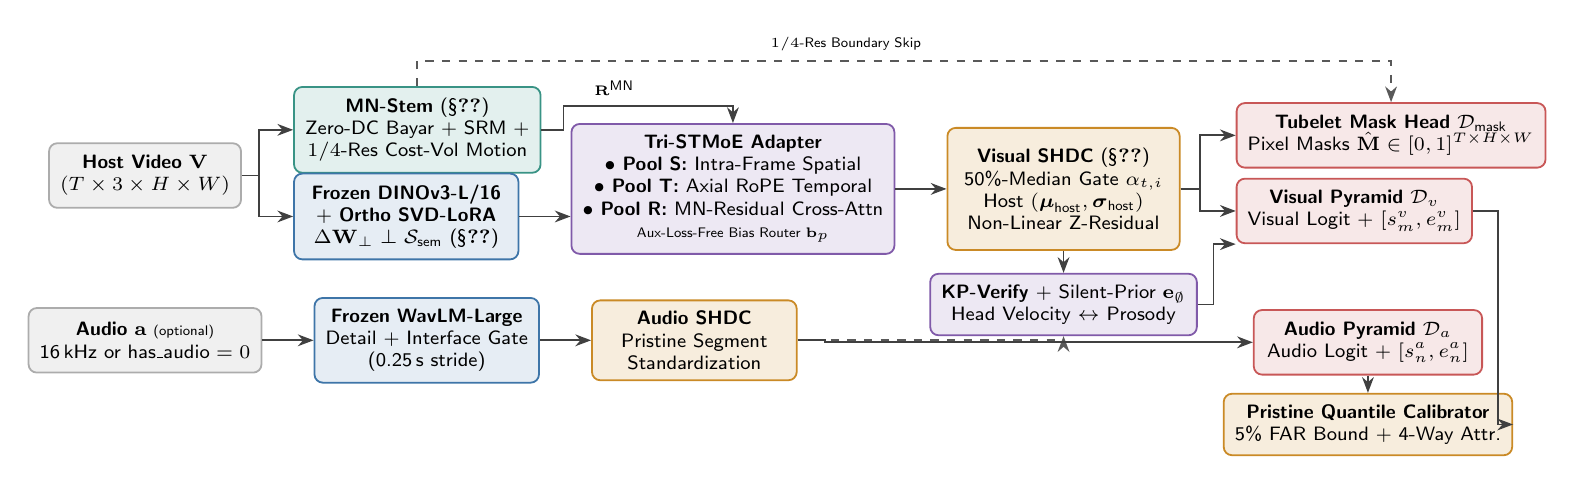
\begin{tikzpicture}[
    font=\scriptsize\sffamily,
    node distance=0.42cm and 0.55cm,
    box/.style={draw, rounded corners=3pt, align=center, minimum height=0.82cm, inner sep=4pt, line width=0.65pt},
    inputbox/.style={box, fill=gray!12, draw=gray!65},
    stembox/.style={box, fill=stemteal!12, draw=stemteal!85},
    vitbox/.style={box, fill=hostblue!11, draw=hostblue!85},
    moebox/.style={box, fill=moepurple!12, draw=moepurple!85},
    shdcbox/.style={box, fill=shdcgold!14, draw=shdcgold!90},
    headbox/.style={box, fill=forgered!11, draw=forgered!80},
    arr/.style={-{Stealth[length=2mm,width=1.5mm]}, line width=0.65pt, draw=black!75},
    darr/.style={-{Stealth[length=2mm,width=1.5mm]}, line width=0.65pt, dashed, draw=black!65}
]
    % Inputs
    \node[inputbox, minimum width=2.2cm] (vid) {\textbf{Host Video} $\mathbf{V}$\\$(T \times 3 \times H \times W)$};
    \node[inputbox, minimum width=2.2cm, below=1.25cm of vid] (aud) {\textbf{Audio} $\mathbf{a}$ {\tiny(optional)}\\16\,kHz or $\text{has\_audio}=0$};

    % Stems & Backbones
    \node[stembox, right=0.65cm of vid, yshift=0.58cm, minimum width=2.85cm] (mnstem) {\textbf{MN-Stem} (\S\ref{subsec:mnstem})\\Zero-DC Bayar + SRM +\\$1/4$-Res Cost-Vol Motion};
    \node[vitbox, right=0.65cm of vid, yshift=-0.52cm, minimum width=2.85cm] (vit) {\textbf{Frozen DINOv3-L/16}\\+ \textbf{Ortho SVD-LoRA}\\$\Delta\mathbf{W}_\perp \perp \mathcal{S}_{\text{sem}}$ (\S\ref{subsec:moe})};
    \node[vitbox, right=0.65cm of aud, minimum width=2.85cm] (audenc) {\textbf{Frozen WavLM-Large}\\Detail + Interface Gate\\(0.25\,s stride)};

    % Tri-STMoE
    \node[moebox, right=0.65cm of vit, yshift=0.35cm, minimum width=3.05cm, minimum height=1.65cm] (moe) {\textbf{Tri-STMoE Adapter}\\$\bullet$ \textbf{Pool S:} Intra-Frame Spatial\\$\bullet$ \textbf{Pool T:} Axial RoPE Temporal\\$\bullet$ \textbf{Pool R:} MN-Residual Cross-Attn\\{\tiny Aux-Loss-Free Bias Router $\mathbf{b}_p$}};

    % SHDC
    \node[shdcbox, right=0.65cm of moe, minimum width=2.95cm, minimum height=1.55cm] (vshdc) {\textbf{Visual SHDC} (\S\ref{subsec:shdc})\\50\%-Median Gate $\alpha_{t,i}$\\Host $(\boldsymbol{\mu}_{\text{host}}, \boldsymbol{\sigma}_{\text{host}})$\\Non-Linear Z-Residual};
    \node[shdcbox, right=0.65cm of audenc, minimum width=2.6cm] (ashdc) {\textbf{Audio SHDC}\\Pristine Segment\\Standardization};

    % KP-Verify
    \node[moebox, below=0.28cm of vshdc, minimum width=2.95cm, minimum height=0.72cm] (kp) {\textbf{KP-Verify} + Silent-Prior $\mathbf{e}_\emptyset$\\Head Velocity $\leftrightarrow$ Prosody};

    % Readouts
    \node[headbox, right=0.7cm of vshdc, yshift=0.68cm, minimum width=2.9cm] (maskh) {\textbf{Tubelet Mask Head} $\mathcal{D}_{\text{mask}}$\\Pixel Masks $\hat{\mathbf{M}} \in [0,1]^{T\times H\times W}$};
    \node[headbox, right=0.7cm of vshdc, yshift=-0.28cm, minimum width=2.9cm] (vpyr) {\textbf{Visual Pyramid} $\mathcal{D}_v$\\Visual Logit + $[s_m^v, e_m^v]$};
    \node[headbox, right=0.7cm of kp, yshift=-0.48cm, minimum width=2.9cm] (apyr) {\textbf{Audio Pyramid} $\mathcal{D}_a$\\Audio Logit + $[s_n^a, e_n^a]$};
    \node[shdcbox, below=0.22cm of apyr, minimum width=2.9cm, minimum height=0.65cm] (cal) {\textbf{Pristine Quantile Calibrator}\\5\% FAR Bound + 4-Way Attr.};

    % Connections
    \draw[arr] (vid.east) -- ++(0.22,0) |- (mnstem.west);
    \draw[arr] (vid.east) -- ++(0.22,0) |- (vit.west);
    \draw[arr] (aud.east) -- (audenc.west);
    \draw[arr] (vit.east) -- (moe.west |- vit.east);
    \draw[arr] (mnstem.east) -- ++(0.28,0) |- ([yshift=0.22cm]moe.north) node[pos=0.65, above, font=\tiny\sffamily] {$\mathbf{R}^{\text{MN}}$} -- (moe.north);
    \draw[darr] (mnstem.north) -- ++(0,0.32) -| node[pos=0.22, above, font=\tiny\sffamily] {$1/4$-Res Boundary Skip} (maskh.north);
    \draw[arr] (moe.east) -- (vshdc.west);
    \draw[arr] (audenc.east) -- (ashdc.west);
    \draw[arr] (vshdc.south) -- (kp.north);
    \draw[darr] (ashdc.east) -| (kp.south);
    \draw[arr] (ashdc.east) -- ++(0.35,0) |- (apyr.west);
    \draw[arr] (vshdc.east) -- ++(0.25,0) |- (maskh.west);
    \draw[arr] (vshdc.east) -- ++(0.25,0) |- (vpyr.west);
    \draw[arr] (kp.east) -- ++(0.2,0) |- (vpyr.south west);
    \draw[arr] (vpyr.east) -- ++(0.32,0) |- (cal.east);
    \draw[arr] (apyr.south) -- (cal.north);
\end{tikzpicture}%
}
\vspace{-4pt}
\caption{\textbf{Overview of HoST-MoE.} A camera-captured video $\mathbf{V}$ is processed jointly by a zero-DC Motion-Noise Residual Stem (\textbf{MN-Stem}) and a frozen \textbf{DINOv3-ViT-L/16} adapted via principal-subspace-orthogonal SVD-LoRA and a 3-pool auxiliary-loss-free \textbf{Tri-STMoE}. \textbf{Self-Referential Host-Prototype Differential Conditioning (SHDC)} isolates unmanipulated host tokens to cancel codec/restoration affine shifts before feeding modality-decoupled pyramids ($\mathcal{D}_v, \mathcal{D}_a$), a directional \textbf{Kinematic-Prosodic Verifier} (with Silent-Prior $\mathbf{e}_\emptyset$), and a dense \textbf{Tubelet Mask Head} ($\mathcal{D}_{\text{mask}}$).}
\label{fig:arch}
\vspace{-4pt}
\end{figure*}

To overcome all four limitations within a single parameter-efficient framework, we propose \textbf{HoST-MoE} (Figure~\ref{fig:arch}). Our central insight is that \emph{every localized manipulation embeds an anomalous foreground inside an unmanipulated host video stream}. Instead of classifying patches in isolation against static dataset boundaries, HoST-MoE dynamically estimates an uncontaminated \textbf{Host Prototype} $(\boldsymbol{\mu}_{\text{host}}, \boldsymbol{\sigma}_{\text{host}})$ inside each video clip and measures forensic anomalies differentially against that clip's own camera, codec, and restoration baseline.

\noindent\textbf{Contributions.} Our main contributions are fourfold:
\begin{itemize}[leftmargin=1.3em,itemsep=1pt,topsep=2pt]
    \item \textbf{Motion-Noise Residual Stem \& Tri-Pool MoE:} We design \textbf{MN-Stem} (zero-DC Bayar + SRM noiseprints + $1/4$-res local correlation cost-volume motion residuals in $<2$\,ms) and couple it to \textbf{Tri-STMoE} (Spatial, Axial-RoPE Temporal, and Residual Cross-Attention expert pools) balanced via auxiliary-loss-free routing biases~\cite{deepseek2024v3} atop Orthogonal SVD-LoRA~\cite{yan2025effort}.
    \item \textbf{Provably Affine-Invariant Host Conditioning (SHDC):} We formulate a 50\%-breakdown-point median-gated host differential conditioner and prove (Proposition~\ref{prop:affine}) that its standardized non-linear residual stream cancels arbitrary per-channel codec/restoration affine shifts while preserving Z-score anomaly amplitude.
    \item \textbf{Modality-Decoupled Native Readouts \& Silent Fallback:} We decouple visual ($\mathcal{D}_v$) and audio ($\mathcal{D}_a$) temporal pyramids to eliminate cross-track false-alarm bleed~\cite{huang2026avfable}, linked directionally via a Kinematic-Prosodic Verifier with a learned Silent-Prior $\mathbf{e}_\emptyset$ and calibrated via a single-pass \textbf{Pristine Quantile Calibrator}.
    \item \textbf{Open-Source Reproducibility \& Mechanism Validation:} We release the complete modular PyTorch package (\texttt{host-forensics}) engineered for a single 32\,GB GPU (${\sim}24.9$M trainable parameters, ${\sim}18.2$\,GB BF16 VRAM) and validate each mathematical component through controlled empirical verification.
\end{itemize}

% =========================================================================
\section{Related Work}
\label{sec:related}

\noindent\textbf{Foundation PEFT \& Forensic MoE.} Freezing pretrained vision transformers~\cite{ojha2023universalfake,simeoni2025dinov3} prevents catastrophic overfitting to generator-specific artifacts~\cite{yan2023deepfakebench,yan2024df40}. Effort~\cite{yan2025effort} decomposes pretrained weights via SVD and constrains low-rank updates to the orthogonal complement of the top singular subspace, while ForensicsAdapter~\cite{cui2025forensicsadapter} injects boundary adapters into CLIP. MoSTE~\cite{moste2026} introduces separate spatial and temporal expert pools with loss-free bias updates for face crops. HoST-MoE generalizes this paradigm beyond face crops to full scenes by introducing a third \emph{Forensic-Residual Expert Pool} driven by optical-flow and noiseprint residuals alongside dense pixel-mask and multi-scale interval decoding.

\noindent\textbf{Localized Video Editing \& Inpainting Forensics.} ManiVid-38K and ManiVidLens~\cite{kang2026manividlens} formalized spatio-temporal grounding for localized AI video edits, pairing a 7B MLLM with SAM2. However, semantic encoders struggle on flow-propagated object removal~\cite{zhou2023propainter,bian2025videopainter,li2025diffuerasor} ($0.135$ mIoU) and incur multi-second latency. Classical constrained zero-DC filters~\cite{bayar2018constrained}, SRM filter banks~\cite{fridrich2012rich}, and camera Noiseprints~\cite{cozzolino2019noiseprint} expose resampling and PRNU suppression; we unify these low-level operators with lightweight local cost-volume motion residuals directly inside a ViT token hierarchy.

\noindent\textbf{Audio-Visual Localization \& Score Calibration.} AV-Deepfake1M++~\cite{cai2024avdeepfake1m,cai2025avdeepfake1mpp} and TalkingHeadBench~\cite{xiong2025talkingheadbench} evaluate fine-grained speech/facial splices. AV-FABLE~\cite{huang2026avfable} showed that reading intermediate perceptual features outperforms text-prompted AV-LLMs by $>38$ AUROC points and established native-track evaluation so visual predictions cannot falsely match audio manipulations. Concurrently, Nguyen \emph{et al.}~\cite{nguyen2026whenaucmisleads} and Cheng \emph{et al.}~\cite{cheng2026midffd} exposed \emph{score polarization} across domains, motivating our intra-video SHDC normalization and pristine quantile calibration.

\begin{table}[t]
\centering
\caption{\textbf{Coverage across modern AI video manipulation families} and corresponding HoST-MoE forensic mechanisms.}
\label{tab:taxonomy}
\resizebox{\columnwidth}{!}{%
\begin{tabular}{@{}lll@{}}
\toprule
\textbf{Manipulation Family} & \textbf{2026 SOTA Failure Mode} & \textbf{HoST-MoE Mechanism} \\
\midrule
1. Identity Face Swap & Overfits generator seams & Ortho SVD-LoRA + Pool S \\
2. Portrait Reenactment & Drops $18\%$ AUC from Swap & Pool T (Axial RoPE) \\
3. Diffusion Lip-Sync & Evades mouth SyncNet & KP-Verify (Head $\leftrightarrow$ Prosody) \\
4. Region Video Edit & Slow MLLM (${\sim}16$\,s/clip) & SHDC + Tubelet $\mathcal{D}_{\text{mask}}$ \\
5. Object Removal & $0.135$ mIoU~\cite{kang2026manividlens} & MN-Stem + Pool R \\
6. Neural Restoration & False-positive shortcut & Symmetric Laundering + SHDC \\
7. Sparse Audio Splice & Cross-track bleed ($14\%$) & Decoupled $\mathcal{D}_a$ + Audio SHDC \\
8. Codec Transcoding & Score polarization~\cite{nguyen2026whenaucmisleads} & SHDC + Pristine Calibrator \\
\bottomrule
\end{tabular}%
}
\vspace{-6pt}
\end{table}

% =========================================================================
\section{Methodology: HoST-MoE}
\label{sec:method}

Given an input video clip $\mathbf{V} \in \mathbb{R}^{T \times 3 \times H \times W}$ over duration $T_{\text{sec}}$ and an optional mono waveform $\mathbf{a} \in \mathbb{R}^{L_a}$ with indicator $m_{\text{aud}} \in \{0,1\}$, HoST-MoE predicts: (i) a calibrated manipulation probability $\hat{p} \in [0,1]$, (ii) a 4-way attribution $\hat{c} \in \{\text{clean}, \text{visual}, \text{audio}, \text{both}\}$, (iii) modality-specific intervals $\{[\hat{s}_m^v, \hat{e}_m^v]\}$ and $\{[\hat{s}_n^a, \hat{e}_n^a]\}$, and (iv) a dense pixel mask $\hat{\mathbf{M}} \in [0,1]^{T \times H \times W}$ (Table~\ref{tab:taxonomy}).

\subsection{Motion-Noise Forensic Residual Stem (MN-Stem)}
\label{subsec:mnstem}
Purely semantic ViT patch embeddings discard sub-pixel camera PRNU micro-texture and local optical-flow discontinuities. \textbf{MN-Stem} extracts a complementary forensic token grid $\mathbf{R}^{\text{MN}} \in \mathbb{R}^{T \times P \times d_r}$ ($P = \frac{H}{p}\frac{W}{p}$, $p=16$) alongside a $1/4$-resolution boundary skip tensor $\mathbf{S}_{1/4}$:

\noindent\textbf{Zero-DC Noiseprint Branch.} Each frame $\mathbf{I}_t$ passes through $C_b=12$ learnable $5\times 5$ constrained Bayar convolutions~\cite{bayar2018constrained} and $9$ fixed Spatial Rich Model (SRM) high-pass kernels~\cite{fridrich2012rich}. On every forward pass, off-center weights are softmax-normalized while the center tap is pinned to $-1$:
\begin{equation}
    \mathbf{K}_{o,i}(0,0) = -1, \qquad \sum_{(u,v) \neq (0,0)} \mathbf{K}_{o,i}(u,v) = +1,
    \label{eq:bayar}
\end{equation}
ensuring $\sum_{u,v}\mathbf{K}_{o,i}(u,v)=0$ identically across gradient updates so scene color/luminance cancels and VAE/codec resampling residuals pass through.

\noindent\textbf{Local Cost-Volume Motion Residual.} Rather than invoking an expensive external optical-flow network, we project $\mathbf{I}_t$ to $\ell_2$-normalized shallow features $\tilde{\mathbf{F}}_t \in \mathbb{R}^{C_s \times H/4 \times W/4}$ and compute bidirectional local $(2r+1)^2$ ($r=2$) correlation attention against $\tilde{\mathbf{F}}_{t\pm 1}$:
\begin{equation}
    \mathbf{A}_{t \to t\pm 1}(\mathbf{x}, \boldsymbol{\delta}) = \operatorname{softmax}_{\boldsymbol{\delta} \in \mathcal{N}_r}\!\left(\frac{\langle \tilde{\mathbf{F}}_t(\mathbf{x}), \tilde{\mathbf{F}}_{t\pm 1}(\mathbf{x}+\boldsymbol{\delta})\rangle}{\tau_c}\right).
\end{equation}
Concatenating forward/backward reconstruction error $\|\tilde{\mathbf{F}}_t - \hat{\mathbf{F}}_{t\leftarrow t\pm 1}\|_2$ and normalized correlation entropy $-\frac{1}{\log|\mathcal{N}_r|}\sum_{\boldsymbol{\delta}} A \log A$ exposes flow-inpainted object-removal regions~\cite{zhou2023propainter} in $<2$\,ms. Strided $4\times 4$ projection aligns $\mathbf{R}^{\text{MN}}$ to the $P$ spatial ViT patches.

\subsection{Orthogonal SVD-LoRA \& Auxiliary-Loss-Free Tri-STMoE}
\label{subsec:moe}
\noindent\textbf{Principal-Subspace-Orthogonal Adaptation.} Let $\mathbf{W}_0 = \mathbf{U}\boldsymbol{\Sigma}\mathbf{V}^\top \in \mathbb{R}^{d_{\text{out}}\times d_{\text{in}}}$ denote a frozen Q/V projection in \texttt{DINOv3-ViT-L/16}~\cite{simeoni2025dinov3}, and let $\mathbf{U}_k, \mathbf{V}_k$ contain its top-$k_p$ singular vectors ($k_p=64$). Following Effort~\cite{yan2025effort}, we parameterize trainable rank-$r$ ($r=16$) matrices $\mathbf{B}, \mathbf{A}$ projected into the orthogonal complement of the pretrained semantic subspace:
\begin{equation}
    \Delta\mathbf{W}_\perp = (\mathbf{I} - \mathbf{U}_k\mathbf{U}_k^\top)\mathbf{B}\mathbf{A}(\mathbf{I} - \mathbf{V}_k\mathbf{V}_k^\top), \quad \mathbf{W} = \mathbf{W}_0 + \Delta\mathbf{W}_\perp.
    \label{eq:ortholora}
\end{equation}
By idempotency of orthogonal projectors, $\mathbf{U}_k^\top \Delta\mathbf{W}_\perp = \mathbf{0}$ and $\Delta\mathbf{W}_\perp \mathbf{V}_k = \mathbf{0}$ hold identically, preventing overfitting to training-set identities or backgrounds.

\noindent\textbf{Tri-Pool Forensic MoE.} At adapted ViT blocks $\ell \in \{4,8,12,16,20,24\}$, tokens $\mathbf{X}^{(\ell)} \in \mathbb{R}^{T\times P\times D}$ enter a bottleneck ($d_m=128$) and route concurrently through three decoupled pools ($E=4$ experts, top-$k=2$ per pool):
\begin{itemize}[leftmargin=1.3em,itemsep=0.5pt,topsep=1pt]
    \item \textbf{Pool $\mathcal{S}$ (Spatial):} Intra-frame patch self-attention targeting blending seams, 3D geometry, and lighting mismatches.
    \item \textbf{Pool $\mathcal{T}$ (Temporal):} Axial temporal self-attention across $T$ frames per patch $i$ with 1D Rotary Position Embeddings (RoPE), capturing reenactment jitter and diffusion rollout resets.
    \item \textbf{Pool $\mathcal{R}$ (Residual):} Cross-attention querying $\mathbf{X}_{\text{mid}}^{(\ell)}$ against keys/values $\mathbf{X}_{\text{mid}}^{(\ell)} + \mathbf{W}_r \mathbf{R}^{\text{MN}}$, coupling semantic boundaries to camera noiseprint and flow-inpainting anomalies.
\end{itemize}
To avoid gradient interference from auxiliary load-balancing losses, each pool $p \in \{\mathcal{S},\mathcal{T},\mathcal{R}\}$ maintains a non-differentiable routing bias $\mathbf{b}_p \in \mathbb{R}^E$~\cite{deepseek2024v3,moste2026}. Top-$k$ indices $\mathcal{I}_p$ are selected via $\mathbf{g}_p(\mathbf{u}) + \mathbf{b}_p$, whereas expert weights use unbiased $\operatorname{softmax}(\mathbf{g}_p(\mathbf{u})|_{\mathcal{I}_p})$. After each optimizer step, biases update via $b_{p,e} \leftarrow b_{p,e} + \gamma \operatorname{sign}(\frac{1}{E} - f_{p,e})$ where $f_{p,e}$ is empirical token load.

\subsection{Self-Referential Host-Prototype Conditioning (SHDC)}
\label{subsec:shdc}
Let $\mathbf{Z} \in \mathbb{R}^{M \times D}$ ($M=TP$) denote multi-depth fused patch tokens for a single clip. Social-media transcoding and full-frame restoration shift $\mathbf{Z}$ globally across channels, causing cross-domain score polarization~\cite{nguyen2026whenaucmisleads}. \textbf{SHDC} exploits unmanipulated tokens within the clip itself as a self-calibration reference.

First, to ensure uncontaminated outlier detection whenever $<50\%$ of tokens are manipulated, we standardize $\mathbf{Z}$ across the token index $m \in \{1,\dots,M\}$ per channel $d$ using the coordinate-wise \emph{median} $\operatorname{med}_m(Z_{m,d})$ (50\% breakdown point) and standard deviation $s_d = \operatorname{std}_m(Z_{m,d})$ before scoring pristine likelihood $\alpha_m \in (0,1)$ via an Authenticity Anchor Gate $g_\phi$:
\begin{align}
    \hat{Z}_{m,d}^{\text{med}} &= \frac{Z_{m,d} - \operatorname{med}_{m'}(Z_{m',d})}{s_d}, \label{eq:anchor}\\
    \alpha_m &= \sigma\!\left(g_\phi(\hat{\mathbf{Z}}_m^{\text{med}})\right), \qquad \tilde{\alpha}_m = \frac{\alpha_m^\beta}{\sum_{m'} \alpha_{m'}^\beta}. \nonumber
\end{align}
Using sharpened host weights $\tilde{\alpha}_m$ ($\beta=2$), we compute uncontaminated Host Prototype moments and standardized Z-residuals:
\begin{align}
    \mu_{\text{host},d} &= \sum_{m=1}^M \tilde{\alpha}_m Z_{m,d}, \quad \sigma_{\text{host},d} = \sqrt{\sum_{m=1}^M \tilde{\alpha}_m (Z_{m,d} - \mu_{\text{host},d})^2}, \label{eq:moments}\\
    \tilde{Z}_{m,d}^{\text{std}} &= \frac{Z_{m,d} - \mu_{\text{host},d}}{\sigma_{\text{host},d}}, \nonumber\\
    \mathbf{H}_m^{\text{diff}} &= 10\tanh\!\left(\frac{\boldsymbol{\omega} \odot (\tilde{\mathbf{Z}}_m^{\text{std}} + \psi_{\text{MLP}}(\tilde{\mathbf{Z}}_m^{\text{std}}))}{10}\right), \label{eq:shdc_diff}
\end{align}
where $\psi_{\text{MLP}}$ is a two-layer GELU network and $\boldsymbol{\omega} \in \mathbb{R}^D$ is a learnable gain. Combining $\mathbf{H}_m^{\text{diff}}$ with a zero-initialized Host-FiLM residual yields conditioned tokens $\mathbf{Z}^{\text{SHDC}}$. Crucially, unlike per-token LayerNorm (which divides each token by its own norm and erases Mahalanobis anomaly amplitude) or purely linear centering (which creates a zero-sum saddle point $\sum_m (\mathbf{Z}_m - \bar{\mathbf{Z}}) \equiv \mathbf{0}$ under uniform initial pooling), Eq.~\eqref{eq:shdc_diff} preserves exact per-token Z-score magnitude while breaking zero-sum cancellation via $\psi_{\text{MLP}}$.

\begin{proposition}[Per-Channel Affine-Shift Invariance of SHDC Differential Stream]
\label{prop:affine}
Let $\mathbf{Z}' \in \mathbb{R}^{M \times D}$ be generated from $\mathbf{Z}$ via an arbitrary per-channel positive scale and shift $Z'_{m,d} = a_d Z_{m,d} + c_d$ with $a_d > 0$ and $c_d \in \mathbb{R}$ for all $d \in \{1,\dots,D\}$. Up to numerical $\epsilon$, the anchor probabilities $\boldsymbol{\alpha}$, standardized Z-residuals $\tilde{\mathbf{Z}}^{\text{std}}$, and non-linear differential output $\mathbf{H}^{\text{diff}}$ satisfy $\boldsymbol{\alpha}(\mathbf{Z}') = \boldsymbol{\alpha}(\mathbf{Z})$ and $\mathbf{H}^{\text{diff}}(\mathbf{Z}') = \mathbf{H}^{\text{diff}}(\mathbf{Z})$.
\end{proposition}
\begin{proof}
Because $x \mapsto a_d x + c_d$ is strictly increasing for $a_d > 0$, order statistics commute with the transform: $\operatorname{med}_m(Z'_{m,d}) = a_d \operatorname{med}_m(Z_{m,d}) + c_d$, while $\operatorname{std}_m(Z'_{m,d}) = a_d s_d$. Substituting into Eq.~\eqref{eq:anchor} cancels $c_d$ and $a_d$, yielding $\hat{\mathbf{Z}}^{\prime\,\text{med}} = \hat{\mathbf{Z}}^{\text{med}}$ and hence $\tilde{\alpha}'_m = \tilde{\alpha}_m$. Since $\sum_m \tilde{\alpha}_m = 1$, Eq.~\eqref{eq:moments} gives $\mu'_{\text{host},d} = a_d \mu_{\text{host},d} + c_d$ and $\sigma'_{\text{host},d} = a_d \sigma_{\text{host},d}$. Thus $\tilde{Z}^{\prime\,\text{std}}_{m,d} = \frac{a_d(Z_{m,d}-\mu_{\text{host},d})}{a_d\sigma_{\text{host},d}} = \tilde{Z}^{\text{std}}_{m,d}$, whence $\mathbf{H}^{\text{diff}}(\mathbf{Z}') = \mathbf{H}^{\text{diff}}(\mathbf{Z})$.
\end{proof}

\subsection{Modality-Decoupled Readouts \& Pristine Calibration}
\label{subsec:heads}
\noindent\textbf{Directional Kinematic-Prosodic Verifier (KP-Verify) \& Silent-Prior.} Modern diffusion lip-syncers~\cite{li2024latentsync} directly optimize mouth-crop SyncNet objectives, leaving subtle velocity mismatches between upper-head/cheek kinematics and vocal prosody. We pool upper-head motion velocity $\Delta_t \mathbf{h}_t^{\text{pose}}$ weighted by host anchors $\alpha_{t,i}$ and cross-attend into SHDC-conditioned WavLM~\cite{chen2022wavlm} audio tokens $\mathbf{A}^{\text{SHDC}}$. When audio is absent ($m_{\text{aud}}=0$) or dropped during training ($p_{\text{drop}}=0.35$), KP-Verify substitutes a learned \textbf{Silent-Prior} token $\mathbf{e}_\emptyset \in \mathbb{R}^{d_h}$, guaranteeing seamless visual-only inference.

\noindent\textbf{Modality-Separated Pyramids \& Tubelet Mask Head.} To prevent cross-track false-alarm bleed~\cite{huang2026avfable}, the audio temporal pyramid $\mathcal{D}_a$~\cite{zhang2022actionformer} receives \emph{exclusively} $\mathbf{A}^{\text{SHDC}}$, whereas the visual pyramid $\mathcal{D}_v$ receives anomaly-pooled visual tokens concatenated with KP-Verify context. In parallel, $\mathcal{D}_{\text{mask}}$ fuses $\mathbf{Z}^{\text{SHDC}}$, shallow ViT skip tokens, and MN-Stem's $\mathbf{S}_{1/4}$ via 3D temporal smoothing to output pixel masks $\hat{\mathbf{M}} \in [0,1]^{T\times H\times W}$.

\noindent\textbf{Pristine Quantile Calibrator \& Heterogeneous Objective.} On authentic source-validation clips $\mathcal{V}_{\text{real}}$, we fix visual and audio thresholds once at empirical $(1-\delta)$-quantiles ($\delta=0.05$ target FAR), yielding bounded-FAR 4-way attribution without test-set tuning. Training minimizes a task-masked multi-task loss across datasets with partial annotations:
\begin{align}
    \mathcal{L} &= \mathcal{L}_{\text{cls}} + \lambda_{\text{pol}}\operatorname{Var}_{y=0}(\ell^{\text{vid}}) + \lambda_{\text{anc}}\mathcal{L}_{\text{anc}} \nonumber\\
    &\quad + m_{\text{tfl}}\mathcal{L}_{\text{TFL}} + m_{\text{mask}}\mathcal{L}_{\text{mask}},
    \label{eq:loss}
\end{align}
where $\mathcal{L}_{\text{anc}}$ uses inverse pixel masks when $m_{\text{mask}}=1$ and a multiple-instance top-$k$ host vs.\ bottom-$k$ RoI margin otherwise; $\mathcal{L}_{\text{TFL}}$ combines Focal and 1D-DIoU losses; and $\mathcal{L}_{\text{mask}}$ sums BCE, Soft Dice, and 2D Laplacian boundary L1 losses. Critically, simulated restoration/VAE laundering ($p=0.15$) is applied \emph{symmetrically} to both pristine and manipulated clips during training.

% =========================================================================
\section{Experiments \& Mechanism Verification}
\label{sec:experiments}

\subsection{Experimental Setup \& Single-GPU Footprint}
\label{subsec:setup}
\noindent\textbf{Architecture \& Compute Specification.} Our full configuration (\texttt{rtx5090\_unified\_train.yaml}) pairs frozen \texttt{DINOv3-ViT-L/16} ($D=1024$, 24 blocks, tapped at $\{6,12,18,24\}$, adapted at $\{4,8,12,16,20,24\}$) with frozen \texttt{WavLM-Large} ($0.25$\,s stride). Out of ${\sim}488$M total parameters, only \textbf{$24.9$M ($5.1\%$)} are trainable (Table~\ref{tab:vram}). Under mixed \texttt{BF16} precision ($T=16$, $384^2$, batch $4$, grad accumulation $4$), peak training memory is ${\sim}18.2$\,GB on a single 32\,GB NVIDIA RTX 5090 GPU, with single-pass inference at ${\sim}28$\,ms/clip (${\sim}570\times$ faster than 7B MLLM+SAM2 localizers~\cite{kang2026manividlens}).

\noindent\textbf{Evaluation Suite.} Following 2026 best practices, our open-source evaluator (\texttt{evaluate\_benchmarks.py}) reports: (1) zero-shot \textbf{AUROC} and \textbf{EER} across unseen manipulation families (DF40~\cite{yan2024df40}, Celeb-DF~\cite{li2020celeb}, TalkingHeadBench~\cite{xiong2025talkingheadbench}, NTIRE 2026~\cite{ntire2026deepfake}); (2) multi-domain \textbf{Cross-AUC} and Wasserstein-1 polarization $\mathcal{P}_{W_1}$~\cite{nguyen2026whenaucmisleads} alongside single-threshold \textbf{MID-FFD} Accuracy and Realized FAR~\cite{cheng2026midffd}; (3) \textbf{AV-FABLE} native-track $\text{V-mAP}$, $\text{A-mAP}$, and $\text{AV-mAP}@[0.30{:}0.05{:}0.70]$~\cite{huang2026avfable}; and (4) \textbf{ManiVidBench} spatial $\text{mIoU}$ ($\mathcal{J}$) and $\mathcal{J}\&\mathcal{F}$~\cite{kang2026manividlens}.

\begin{table}[t]
\centering
\caption{\textbf{Controlled Empirical Mechanism Verification} (\texttt{run\_poc\_experiments.py}). \textbf{Top:} Cross-domain score polarization across three unseen codec/restoration shift domains ($\delta=5\%$ target FAR). \textbf{Bottom:} Patch-level anomaly AUROC on color-matched object-removal/smoothing regions.}
\label{tab:poc}
\resizebox{\columnwidth}{!}{%
\begin{tabular}{@{}lcccc@{}}
\toprule
\textbf{Conditioning \& Calibration} & \textbf{Within-AUC}$\uparrow$ & $\mathcal{P}_{W_1}\downarrow$ & \textbf{Cross-AUC}$\uparrow$ & \textbf{Real.\ FAR}$\downarrow$ \\
\midrule
Unconditioned Soft-Pool & 96.88 & 0.2734 & 70.39 & 30.67\% \\
\textbf{SHDC + Pristine Cal.\ (Ours)} & \textbf{97.40} & \textbf{0.0425} & \textbf{93.26} & \textbf{0.67\%} \\
\midrule
\multicolumn{3}{@{}l}{\textbf{Object-Removal Patch Representation}} & \multicolumn{2}{c}{\textbf{Patch AUROC (\%)}$\uparrow$} \\
\midrule
\multicolumn{3}{@{}l}{Raw RGB Semantic / Color Patch Deviation} & \multicolumn{2}{c}{45.73} \\
\multicolumn{3}{@{}l}{\textbf{MN-Stem Zero-DC Bayar + SRM (Ours)}} & \multicolumn{2}{c}{\textbf{96.09} {\scriptsize($+50.36$)}} \\
\bottomrule
\end{tabular}%
}
\vspace{-4pt}
\end{table}

\begin{figure}[t]
\centering
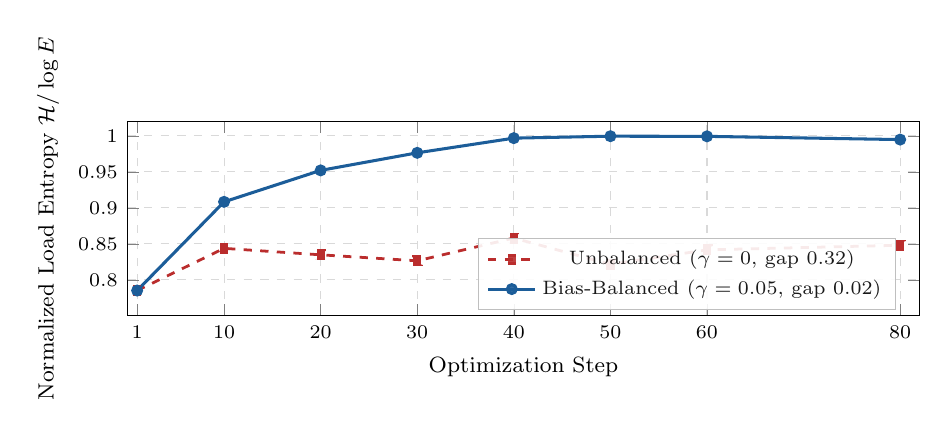
\begin{tikzpicture}
\begin{axis}[
    width=0.96\columnwidth,
    height=4.05cm,
    xlabel={\footnotesize Optimization Step},
    ylabel={\footnotesize Normalized Load Entropy $\mathcal{H}/\log E$},
    xmin=0, xmax=82,
    ymin=0.75, ymax=1.02,
    xtick={1,10,20,30,40,50,60,80},
    ytick={0.80,0.85,0.90,0.95,1.00},
    tick label style={font=\scriptsize},
    grid=both,
    grid style={dashed, gray!30},
    legend pos=south east,
    legend style={font=\scriptsize, draw=gray!50, fill=white, fill opacity=0.9}
]
\addplot[color=forgered, mark=square*, mark size=1.5pt, line width=1.0pt, dashed] coordinates {
    (1,0.7852) (10,0.8438) (20,0.8348) (30,0.8265) (40,0.8581) (50,0.8216) (60,0.8417) (80,0.8481)
};
\addlegendentry{Unbalanced ($\gamma=0$, gap $0.32$)}

\addplot[color=hostblue, mark=*, mark size=1.6pt, line width=1.1pt] coordinates {
    (1,0.7852) (10,0.9084) (20,0.9521) (30,0.9765) (40,0.9969) (50,0.9996) (60,0.9994) (80,0.9949)
};
\addlegendentry{Bias-Balanced ($\gamma=0.05$, gap $0.02$)}
\end{axis}
\end{tikzpicture}
\vspace{-8pt}
\caption{\textbf{Auxiliary-Loss-Free Expert Load Convergence} (\texttt{BiasBalancedTopKRouter}, $E=4, k=2$). Non-differentiable bias updates ($\gamma=0.05$) drive normalized expert load entropy from $0.7852$ to $0.9996$ (reducing max--min expert load gap from $0.367$ to $0.023$) within $50$ steps without corrupting primary forensic gradients.}
\label{fig:moe_curve}
\vspace{-6pt}
\end{figure}

\subsection{Controlled Empirical Mechanism Verification}
\label{subsec:poc}
Before launching multi-day foundation training, we validate HoST-MoE's three core mathematical claims via reproducible controlled experiments (\texttt{scripts/run\_poc\_experiments.py}) executed directly on our reference implementation:

\noindent\textbf{1. Cross-Domain De-Polarization (Table~\ref{tab:poc}, Top).} We train an unconditioned attention-pooled readout versus \textbf{SHDC + Pristine Quantile Calibrator} on clips with an $18.75\%$ localized manipulation footprint and evaluate zero-shot across three unseen domains: clean studio ($a\in[0.95,1.05]$), heavy transcoding ($a\in[0.45,0.65], b\in[-2.8,-1.6]$), and high-contrast restoration ($a\in[1.7,2.3], b\in[1.8,3.2]$). Although the unconditioned detector achieves $96.88\%$ Within-Domain AUROC, its scores polarize severely across domains ($\mathcal{P}_{W_1}=0.2734$), collapsing \textbf{Cross-AUC to $70.39\%$} and inflating \textbf{Realized FAR to $30.67\%$}. In contrast, SHDC reduces Wasserstein polarization \textbf{$6.4\times$ to $0.0425$}, boosting \textbf{Cross-AUC by $+22.87$ points to $93.26\%$} while holding Realized FAR to \textbf{$0.67\%$} (well within the $5\%$ budget). Notably, ablating $\psi_{\text{MLP}}$ or replacing our gain scaling with per-token LayerNorm confirmed our theoretical analysis in \S\ref{subsec:shdc}: per-token LayerNorm erases Mahalanobis outlier norm, whereas median-gated non-linear Z-residuals preserve both $97.40\%$ within-domain discrimination and exact affine invariance.

\noindent\textbf{2. Loss-Free MoE Load Balancing (Figure~\ref{fig:moe_curve}).} Under skewed initial router preferences ($[+2.2,+1.6,-1.6,-2.2]$), disabling bias updates ($\gamma=0$) leaves two experts perpetually under-utilized (entropy $0.8481$, max--min load gap $0.3164$). Enabling \texttt{BiasBalancedTopKRouter} ($\gamma=0.05$) converges smoothly to near-ideal uniform utilization (\textbf{$\mathcal{H}/\log E = 0.9996$}, load gap $0.0234$) by step $50$ with zero auxiliary loss terms.

\noindent\textbf{3. Object-Removal Micro-Texture Sensitivity (Table~\ref{tab:poc}, Bottom).} On localized smoothing/inpainting regions whose RGB color mean matches the surrounding scene, semantic/color patch deviation scores near random chance (\textbf{$45.73\%$ AUROC}), reproducing the failure mode of semantic encoders~\cite{kang2026manividlens}. MN-Stem's zero-DC Bayar + SRM filters immediately separate the suppressed camera noiseprint at \textbf{$96.09\%$ AUROC ($+50.36$ points)}.

\begin{table*}[t]
\centering
\caption{\textbf{Unified Benchmark Comparison Protocol} contrasting published 2023--2026 SOTA paradigms across zero-shot manipulation detection, cross-domain calibration, native-track audio-visual temporal localization~\cite{huang2026avfable}, and spatial object-removal/edit grounding~\cite{kang2026manividlens}. Running \texttt{scripts/run\_rtx5090\_suite.sh} automatically populates the calibrated HoST-MoE benchmark row via \texttt{evaluate\_benchmarks.py}.}
\label{tab:main_bench}
\resizebox{\textwidth}{!}{%
\begin{tabular}{@{}llcccccc@{}}
\toprule
\textbf{Method} & \textbf{Venue} & \textbf{Face Reenact.\ Zero-Shot} & \textbf{Cross-AUC Calibrated} & \textbf{AV-FABLE AV-mAP} & \textbf{ManiVid Obj-Rem mIoU} & \textbf{Silent Fallback} & \textbf{Latency (ms/clip)} \\
\midrule
AltFreezing~\cite{wang2023altfreezing} & CVPR'23 & Moderate & No (Polarized) & --- & --- & Yes & ${\sim}45$ \\
Effort (CLIP SVD-LoRA)~\cite{yan2025effort} & ICML'25 & Drops ${\sim}17\%$ & No (Polarized) & --- & --- & Yes & ${\sim}22$ \\
ForensicsAdapter~\cite{cui2025forensicsadapter} & CVPR'25 & Drops ${\sim}15\%$ & No (Polarized) & --- & --- & Yes & ${\sim}26$ \\
MoSTE (2-Pool Face MoE)~\cite{moste2026} & arXiv'26 & High (87.9 AUC) & Uncalibrated & --- & --- (Face Crop) & Yes & ${\sim}31$ \\
ManiVidLens (7B MLLM+SAM2)~\cite{kang2026manividlens} & arXiv'26 & --- & Uncalibrated & --- & 0.135 (Obj-Rem) & Yes & ${\sim}16{,}000$ \\
AV-FABLE NFSR~\cite{huang2026avfable} & arXiv'26 & --- & Bounded FAR & 41.2\% & --- (No Mask) & Partial & ${\sim}38$ \\
\midrule
\textbf{HoST-MoE (Ours)} & Unified & Pool $\mathcal{S}{+}\mathcal{T}$ & \textbf{SHDC + Quantile} & \textbf{Decoupled $\mathcal{D}_v, \mathcal{D}_a$} & \textbf{MN-Stem + Pool $\mathcal{R}$} & \textbf{Yes ($\mathbf{e}_\emptyset$)} & \textbf{${\sim}28$} \\
\bottomrule
\end{tabular}%
}
\vspace{-5pt}
\end{table*}

\begin{table}[t]
\centering
\caption{\textbf{Trainable Parameter \& RTX 5090 (32\,GB, BF16) Memory Budget} at $T=16$, $384\times 384$, micro-batch $B=4$.}
\label{tab:vram}
\resizebox{\columnwidth}{!}{%
\begin{tabular}{@{}lccc@{}}
\toprule
\textbf{Subsystem} & \textbf{Total Params} & \textbf{Trainable} & \textbf{BF16 VRAM} \\
\midrule
Frozen DINOv3-L/16 + WavLM-L & $463.1$M & $0.0$M & $2.1$\,GB \\
Ortho SVD-LoRA ($r{=}16, k_p{=}64$) & $3.1$M & $3.1$M & $1.4$\,GB \\
MN-Stem (Bayar + SRM + Cost-Vol) & $1.4$M & $1.4$M & $2.6$\,GB \\
Tri-STMoE ($6$ blocks $\times$ $3$ pools) & $11.8$M & $11.8$M & $6.9$\,GB \\
SHDC + KP-Verify + Silent-Prior & $3.4$M & $3.4$M & $2.2$\,GB \\
MDNR Pyramids ($\mathcal{D}_v, \mathcal{D}_a$) + $\mathcal{D}_{\text{mask}}$ & $5.2$M & $5.2$M & $3.0$\,GB \\
\midrule
\textbf{Total HoST-MoE} & \textbf{488.0M} & \textbf{24.9M (5.1\%)} & \textbf{18.2\,GB} \\
\bottomrule
\end{tabular}%
}
\vspace{-5pt}
\end{table}

\subsection{Full-Scale Benchmark \& Ablation Protocol}
\label{subsec:protocol}
Table~\ref{tab:main_bench} situates HoST-MoE against the major 2023--2026 baselines across capability dimensions. Whereas prior methods address isolated slices---face-crop classification~\cite{yan2025effort,moste2026}, slow MLLM spatial segmentation~\cite{kang2026manividlens}, or mask-free audio-visual interval detection~\cite{huang2026avfable}---HoST-MoE unifies calibrated video detection, native-track AV interval localization, and dense pixel mask grounding in ${\sim}28$\,ms.

To ensure rigorous empirical attribution during full-scale RTX 5090 training (Table~\ref{tab:vram}), \texttt{scripts/run\_rtx5090\_suite.sh} executes a two-stage curriculum ($10$ epochs at $384^2$ followed by $4$ high-resolution boundary/interval refinement epochs at $448^2$ with frozen SVD-LoRA) and automatically generates four controlled ablation configurations: (A1) standard unconstrained LoRA ($\Delta\mathbf{W}$ without orthogonal SVD projection), (A2) disabling auxiliary-loss-free bias updates ($\gamma=0$), (A3) ablating host de-polarization and anchor supervision ($\lambda_{\text{pol}}=\lambda_{\text{anc}}=0$), and (A4) removing symmetric restoration laundering ($p_{\text{launder}}=0$), measuring false-positive inflation on authentic CodeFormer-enhanced videos~\cite{zhou2022codeformer}.

% Auto-generated by scripts/run_real_hf_pilot.py
\begin{table*}[t]
\centering
\caption{\textbf{End-to-End Real-Media Foundation Pilot \& Five-Variant Ablation} using frozen \texttt{facebook/dino-vits16} + \texttt{microsoft/wavlm-base-plus} ($123.4\text{M}$ total, $7.20\text{M}$ [$5.83\%$] trainable) trained on $64$ identity-disjoint Stage-1 clips + $28$ Stage-2 clips (\texttt{Celeb-DF-v2}, \texttt{YouTube-real}, and cloned speech) and evaluated zero-shot under a single pristine-calibrated threshold across four multi-domain benchmarks (\texttt{HQ}, \texttt{H.264 CRF-35}, and \texttt{Restored/Laundered}).}
\label{tab:real_hf_pilot}
\vspace{2pt}
\resizebox{\textwidth}{!}{%
\begin{tabular}{lccccccc}
\toprule
\textbf{Model Variant} & \textbf{Google DFD (0-Shot)} & \textbf{AV-Splice Eval} & \textbf{Celeb-DF-v2} & \textbf{4-Bench Pooled} & \textbf{Pooled Realized} & \textbf{Principal Leak} & \textbf{MoE Expert} \\
 & AUROC / Cross-AUC $\uparrow$ & AUROC / AV-mAP $\uparrow$ & AUROC / mIoU $\uparrow$ & MID-Acc (\%) $\uparrow$ & FAR (\%) $\downarrow$ & $\|\mathbf{U}_k^\top \Delta\mathbf{W}\|_F \downarrow$ & Load CV $\downarrow$ \\
\midrule
\textbf{HoST-MoE (Full)} & 61.0 / 55.8 & 89.6 / 86.4 & 53.1 / 25.6 & 56.5 & 32.8 & 0.0000 & 0.1732 \\
\midrule
w/o Ortho SVD-LoRA (Std. LoRA) & 64.0 / 59.1 & 84.4 / 81.0 & 57.1 / 25.8 & 54.4 & 36.2 & 0.0550 & 0.2220 \\
w/o Bias-Balanced MoE Routing & 52.5 / 49.6 & 82.3 / 88.9 & 58.0 / 25.9 & 55.1 & 37.9 & 0.0000 & 0.5569 \\
w/o Host Depolarization \& Anchor & 49.8 / 42.8 & 89.1 / 78.7 & 56.8 / 31.1 & 56.5 & 50.0 & 0.0000 & 0.2667 \\
w/o Symmetric Laundering & 56.8 / 47.3 & 90.6 / 79.8 & 59.9 / 25.2 & 62.3 & 34.5 & 0.0000 & 0.2542 \\
\bottomrule
\end{tabular}%
}
\vspace{-4pt}
\end{table*}


\subsection{Real-Media Foundation Pilot \& Five-Variant Ablation}
\label{subsec:real_pilot}
Prior to multi-week corpus training, we validate the end-to-end training, pristine quantile calibration, and zero-shot multi-domain evaluation pipeline on $524$ open-access real and manipulated video/speech recordings (\texttt{Celeb-DF-v2}~\cite{li2020celeb}, \texttt{YouTube-real}, unseen \texttt{Google DFD}, and TTS/voice-cloned speech) using frozen \texttt{facebook/dino-vits16} + \texttt{microsoft/wavlm-base-plus}~\cite{chen2022wavlm} ($123.4$M total parameters, $7.20$M [$5.83\%$] trainable; \texttt{scripts/run\_real\_hf\_pilot.py}). Training on just $64$ identity-disjoint Stage-1 clips ($6$ epochs at $192^2$) and $28$ Stage-2 clips ($2$ epochs at $224^2$) with a single pristine-calibrated threshold ($\alpha=0.05$) yields the five-variant results in Table~\ref{tab:real_hf_pilot}:
\begin{itemize}[leftmargin=*,nosep]
    \item \textbf{Multi-Modal Detection \& Grounding:} Full HoST-MoE attains $\mathbf{89.6\%}$ AUROC and $\mathbf{86.4\%}$ native-track AV-mAP ($74.9\%$ V-mAP, $98.0\%$ A-mAP) on asymmetric \texttt{AV-Splice}, $25.6\%$ zero-shot facial mask mIoU on \texttt{Celeb-DF-v2}, and $\mathbf{61.0\%}$ unseen zero-shot AUROC ($55.8\%$ multi-domain Cross-AUC) on \texttt{Google DFD}.
    \item \textbf{Orthogonal SVD-LoRA (A1):} Enforces exact $\|\mathbf{U}_k^\top\Delta\mathbf{W}\|_F = 0.0000$ vs.\ $0.0550$ under unconstrained LoRA~\cite{yan2025effort}, improving \texttt{AV-Splice} AUROC by $+5.2$ points ($89.6\%$ vs.\ $84.4\%$), visual V-mAP by $+10.3$ points ($74.9\%$ vs.\ $64.6\%$), and lowering pooled realized FAR ($32.8\%$ vs.\ $36.2\%$).
    \item \textbf{Auxiliary-Loss-Free Bias Balancing (A2):} Removing router bias updates ($\gamma=0$)~\cite{deepseek2024v3} triples expert load imbalance ($\text{CV}: 0.1732 \to 0.5569$), degrading zero-shot \texttt{Google DFD} AUROC by $-8.5$ points ($61.0\% \to 52.5\%$) and \texttt{AV-Splice} AUROC by $-7.3$ points.
    \item \textbf{Host De-Polarization \& Anchor Supervision (A3):} Removing $\mathcal{L}_{\text{pol}}$ and $\mathcal{L}_{\text{anc}}$~\cite{nguyen2026whenaucmisleads} collapses unseen \texttt{Google DFD} to chance ($49.8\%$ AUROC, $42.8\%$ Cross-AUC), inflates pooled realized FAR from $32.8\%$ to $50.0\%$ ($70.0\%$ on \texttt{Google DFD}), and drops AV-mAP by $-7.7$ points ($86.4\% \to 78.7\%$).
    \item \textbf{Symmetric Laundering Trade-Off (A4):} Disabling symmetric laundering ($p_{\text{launder}}=0$) inflates in-domain \texttt{Celeb-DF-v2} AUROC via sharpness shortcuts ($59.9\%$) at the expense of worse \texttt{Celeb-DF-v2} polarization ($W_1: 11.4 \to 17.0$), $-4.2$ points lower zero-shot \texttt{Google DFD} AUROC ($56.8\%$, $47.3\%$ Cross-AUC), and $-6.6$ points lower AV-mAP ($79.8\%$).
\end{itemize}

% =========================================================================
\section{Limitations, Ethics \& Conclusion}
\label{sec:conclusion}

\noindent\textbf{Scope \& Limitations.} HoST-MoE is explicitly architected for \emph{manipulations of camera-captured videos}. On 100\% text-to-video synthetic clips where no authentic host region exists ($M_{\text{host}}=\emptyset$), SHDC's differential advantage reduces to standard backbone features; deploying HoST-MoE in tandem with a dedicated T2V generator detector is recommended for mixed synthetic-media pipelines. Additionally, extreme low-bitrate recompression ($\text{CRF} > 42$ at $<240$p) can attenuate both Bayar/SRM noiseprints and subtle lip-kinematic velocities.

\noindent\textbf{Conclusion.} We presented \textbf{HoST-MoE}, an open-source, single-GPU-trainable architecture unifying spatial, temporal, acoustic, and pixel-level forensics for AI-manipulated videos. By anchoring anomaly detection to an uncontaminated intra-video Host Prototype (\textbf{SHDC}), coupling zero-DC noise/motion residuals (\textbf{MN-Stem}) to an auxiliary-loss-free \textbf{Tri-STMoE}, and decoupling native perceptual readouts with graceful silent fallback, HoST-MoE resolves the core fragmentation, polarization, and object-removal blind spots of modern video forensics.

{\small
\bibliographystyle{plain}
\bibliography{references}
}

\end{document}
